\documentclass[12pt, UTF8]{ctexart}

%% 页面设置
\usepackage{geometry}
\geometry{a4paper, margin=1.2in}
\usepackage{fancyhdr}
\pagestyle{plain}
\usepackage{enumitem} % 改善列表间距 \setlength{\itemsep}{-0.1cm}

%% 符号、字体
\usepackage{amsmath, amssymb, amsthm, bm, mathrsfs}
% \usepackage{fixdif} % 微分符号 https://zhuanlan.zhihu.com/p/521009044

%% 引入图片、绘制矢量图
\usepackage{graphicx}
\graphicspath{ 
  {./images/}
  {../images/}
}
\usepackage{float}
\usepackage{caption}
\usepackage{subcaption}
\usepackage[dvipsnames]{xcolor}
\usepackage{tikz, pgf}
\usetikzlibrary{automata, positioning, arrows}

%% 代码块
\usepackage{listings}
% \setmonofont{Monaco}[AutoFakeBold]

%% 链接、索引
\usepackage[colorlinks,linkcolor=black]{hyperref}
\usepackage{makeidx}
\makeindex
\bibliographystyle{plain}

%% 定理环境 https://ask.latexstudio.net/ask/article/647.html
\newtheoremstyle{mystyle}                                % 样式名
  {}                                                     % 上方间距
  {}                                                     % 下方间距
  {\normalfont}                                          % 主体字体
  {}                                                     % 缩进量
  {\bfseries}                                            % 标题字体
  {}                                                     % 标题后的点
  { }                                                    % 标题后的空白符
  {\underline{\thmname{#1}\thmnumber{#2}\thmnote{(#3)}}} % 标题样式
\theoremstyle{mystyle}

% \newtheorem{<环境名>}[<共享计数器>]{<定理头文本>}
\newtheorem{theorem}{定理}[section]
\newtheorem{lemma}{引理}[section]
\renewcommand{\proofname}{证明}

\makeatletter % use at mark
\renewenvironment{proof}[1][\proofname]{\par
  \pushQED{\qed}%
  \normalfont \topsep6\p@\@plus6\p@\relax
  \trivlist
  \item[\hskip\labelsep
        \itshape
    {\bf\underline{#1}}]\ignorespaces
    % {\bf\underline{#1}\@addpunct{.}}]\ignorespaces
}{
  \popQED\endtrivlist\@endpefalse
}
\providecommand{\proofname}{Proof}
\makeatother % end at mark

\usepackage{etoolbox}
\makeatletter
\patchcmd{\l@section}
  {\hfil}
  {\leaders\hbox{\normalfont$\m@th\mkern \@dotsep mu\hbox{.}\mkern \@dotsep mu$}\hfill}
  {}{}
\makeatother

\usepackage{framed}
\definecolor{shadecolor}{RGB}{241, 241, 255}
\newcounter{problemname}
\newenvironment{problem}{\begin{shaded}\stepcounter{problemname}\par\noindent\textbf{题目\arabic{problemname}. }}{\end{shaded}\par}
\newenvironment{solution}{\par\noindent\textbf{答. }}{\par}
\newenvironment{note}{\par\noindent\textbf{题目\arabic{problemname}的注记. }}{\par}

\title{%
  第十八届长沙理工大学ACM程序设计竞赛\\
  \large 验题报告\\}
\author{Kenshin2438}
\date{\today}

\begin{document}

\maketitle
\pagenumbering{roman}
\tableofcontents
\newpage

\pagenumbering{arabic}
\section{不玩原神的请划走}

分类讨论,需要注意的是\textbf{使用64位整数存储结果}。

\section{会长的任务}
这是一道杂糅了\textbf{动态规划}和\textbf{数据结构(线段树/分块)}的题,在\textbf{时间复杂度分析}上也需要一定的经验。
考虑到它的数论背景(欧拉函数),对于此前未接触过算法竞赛(数论)的参赛选手,\textbf{筛法}可能也会有一定的难度。

DP的部分比较简单,对于前$i$个,只需要考虑第$i-1$个元素是否选择,以此转移。数据结构部分有两种维护方式:
\begin{enumerate}[noitemsep]
  \item SegmentTree,维护当前区间左右侧选或者不选的DP值。$\mathcal{O}((n+q)\log{n})$
  \item 分块,对于每个块内部暴力跑DP,块外也通过DP求得答案。$\mathcal{O}(n\sqrt{n})$
\end{enumerate}

关于取欧拉函数值($a[i]=\varphi(a[i])$)的操作,每个数会在$\mathcal{O}(\log{N})$内变成$1$,因此可以直接暴力更改。当一个连续段都变成$1$后,对于此连续段的取欧拉函数的操作已经不用执行。

\section{挤水泡}

搜索,注意剪枝。

\section{体测排队}

逆序对计数,由于数据范围小,维护每个高度的人数即可。

\section{学妹的问题}

组合数学/动态规划。\par
一方面,可以直接通过组合数学的知识得到答案;另一方面,通过分析数组长度从$n-1$到$n$的变化也能求解。

\[
  ans(n) = ans(n-1)\times n + (\sum_{i=1}^{n-1}i)\times (n-1)!
\]

\begin{enumerate}[noitemsep]
  \item $n-1$长的排列形成了$n$个间隔;
  \item 新加入的数字$n$可以和前$n-1$个数形成逆序对。
\end{enumerate}

\section{需要计算 114514 次的矩阵乘法}

区间DP。

\section{n有多大?整个采购部放不下!}

(散列表/离散化)+(动态规划/直接求值)。基本思路同第4题。

\section{神秘的公司}

排序,重点在排序的比较函数上。

\section{杜学长的烦恼(一)}

\begin{enumerate}[noitemsep]
  \item 维护$c,c\times timestamp$,历史和问题(SegmentTree/FenwickTree)
  \item 维护$a$,区间覆盖(SegmentTree)
\end{enumerate}

时间复杂度上,如果放在同一个线段树中,为$\mathcal{O}(n\log{n})$;反之分开维护则为$\mathcal{O}(n\log^2{n})$。转成离线,用ChtollyTree维护区间也行。\par
PS:题目来自2022CCPC广州站B题。对于本题的区间覆盖,本人更倾向于\textbf{时间复杂度为$\mathcal{O}(n\log^2 n)$但运行效率接近$\mathcal{O}(n\log n)$}。

\section{杜学长的烦恼(二)}

主席树/分块bitset\par
分块bitset的方式。出现次数为奇数可以转换成\textbf{奇数个$1$异或结果为$1$},最小的数转换成\textbf{从小到大第一个为$1$的比特位}。\par
\texttt{std::bitset}中,$N$比特异或的时间复杂度为$\mathcal{O}(\frac{N}{\epsilon})$,$N$比特\texttt{\_Find\_first}时间复杂度相同。一般而言我们认为$\epsilon=32$。但是通过手写bitset或是提高优化等级,$\epsilon$会更大。此外,由于空间复杂度过高,我们可以通过分块解决(注意,此处的分块并不是为了\textbf{空间换时间},而是相反,因此需要特别注意分块的大小)。\par
在验题代码中,\texttt{bitset}代码来自\Hurl{https://nyaannyaan.github.io/library}

\section{杜学长的“烦恼”(三)}

简单思维,出现次数最多的字符字串,其首字符的出现了同样的次数。因此答案为\textbf{原始字符串中,出现最多的字符的出现次数}。

\section{这可能是一道签到题?}

打表/Miller-Rabin Primality Test

\begin{figure}[H]
  \centering
  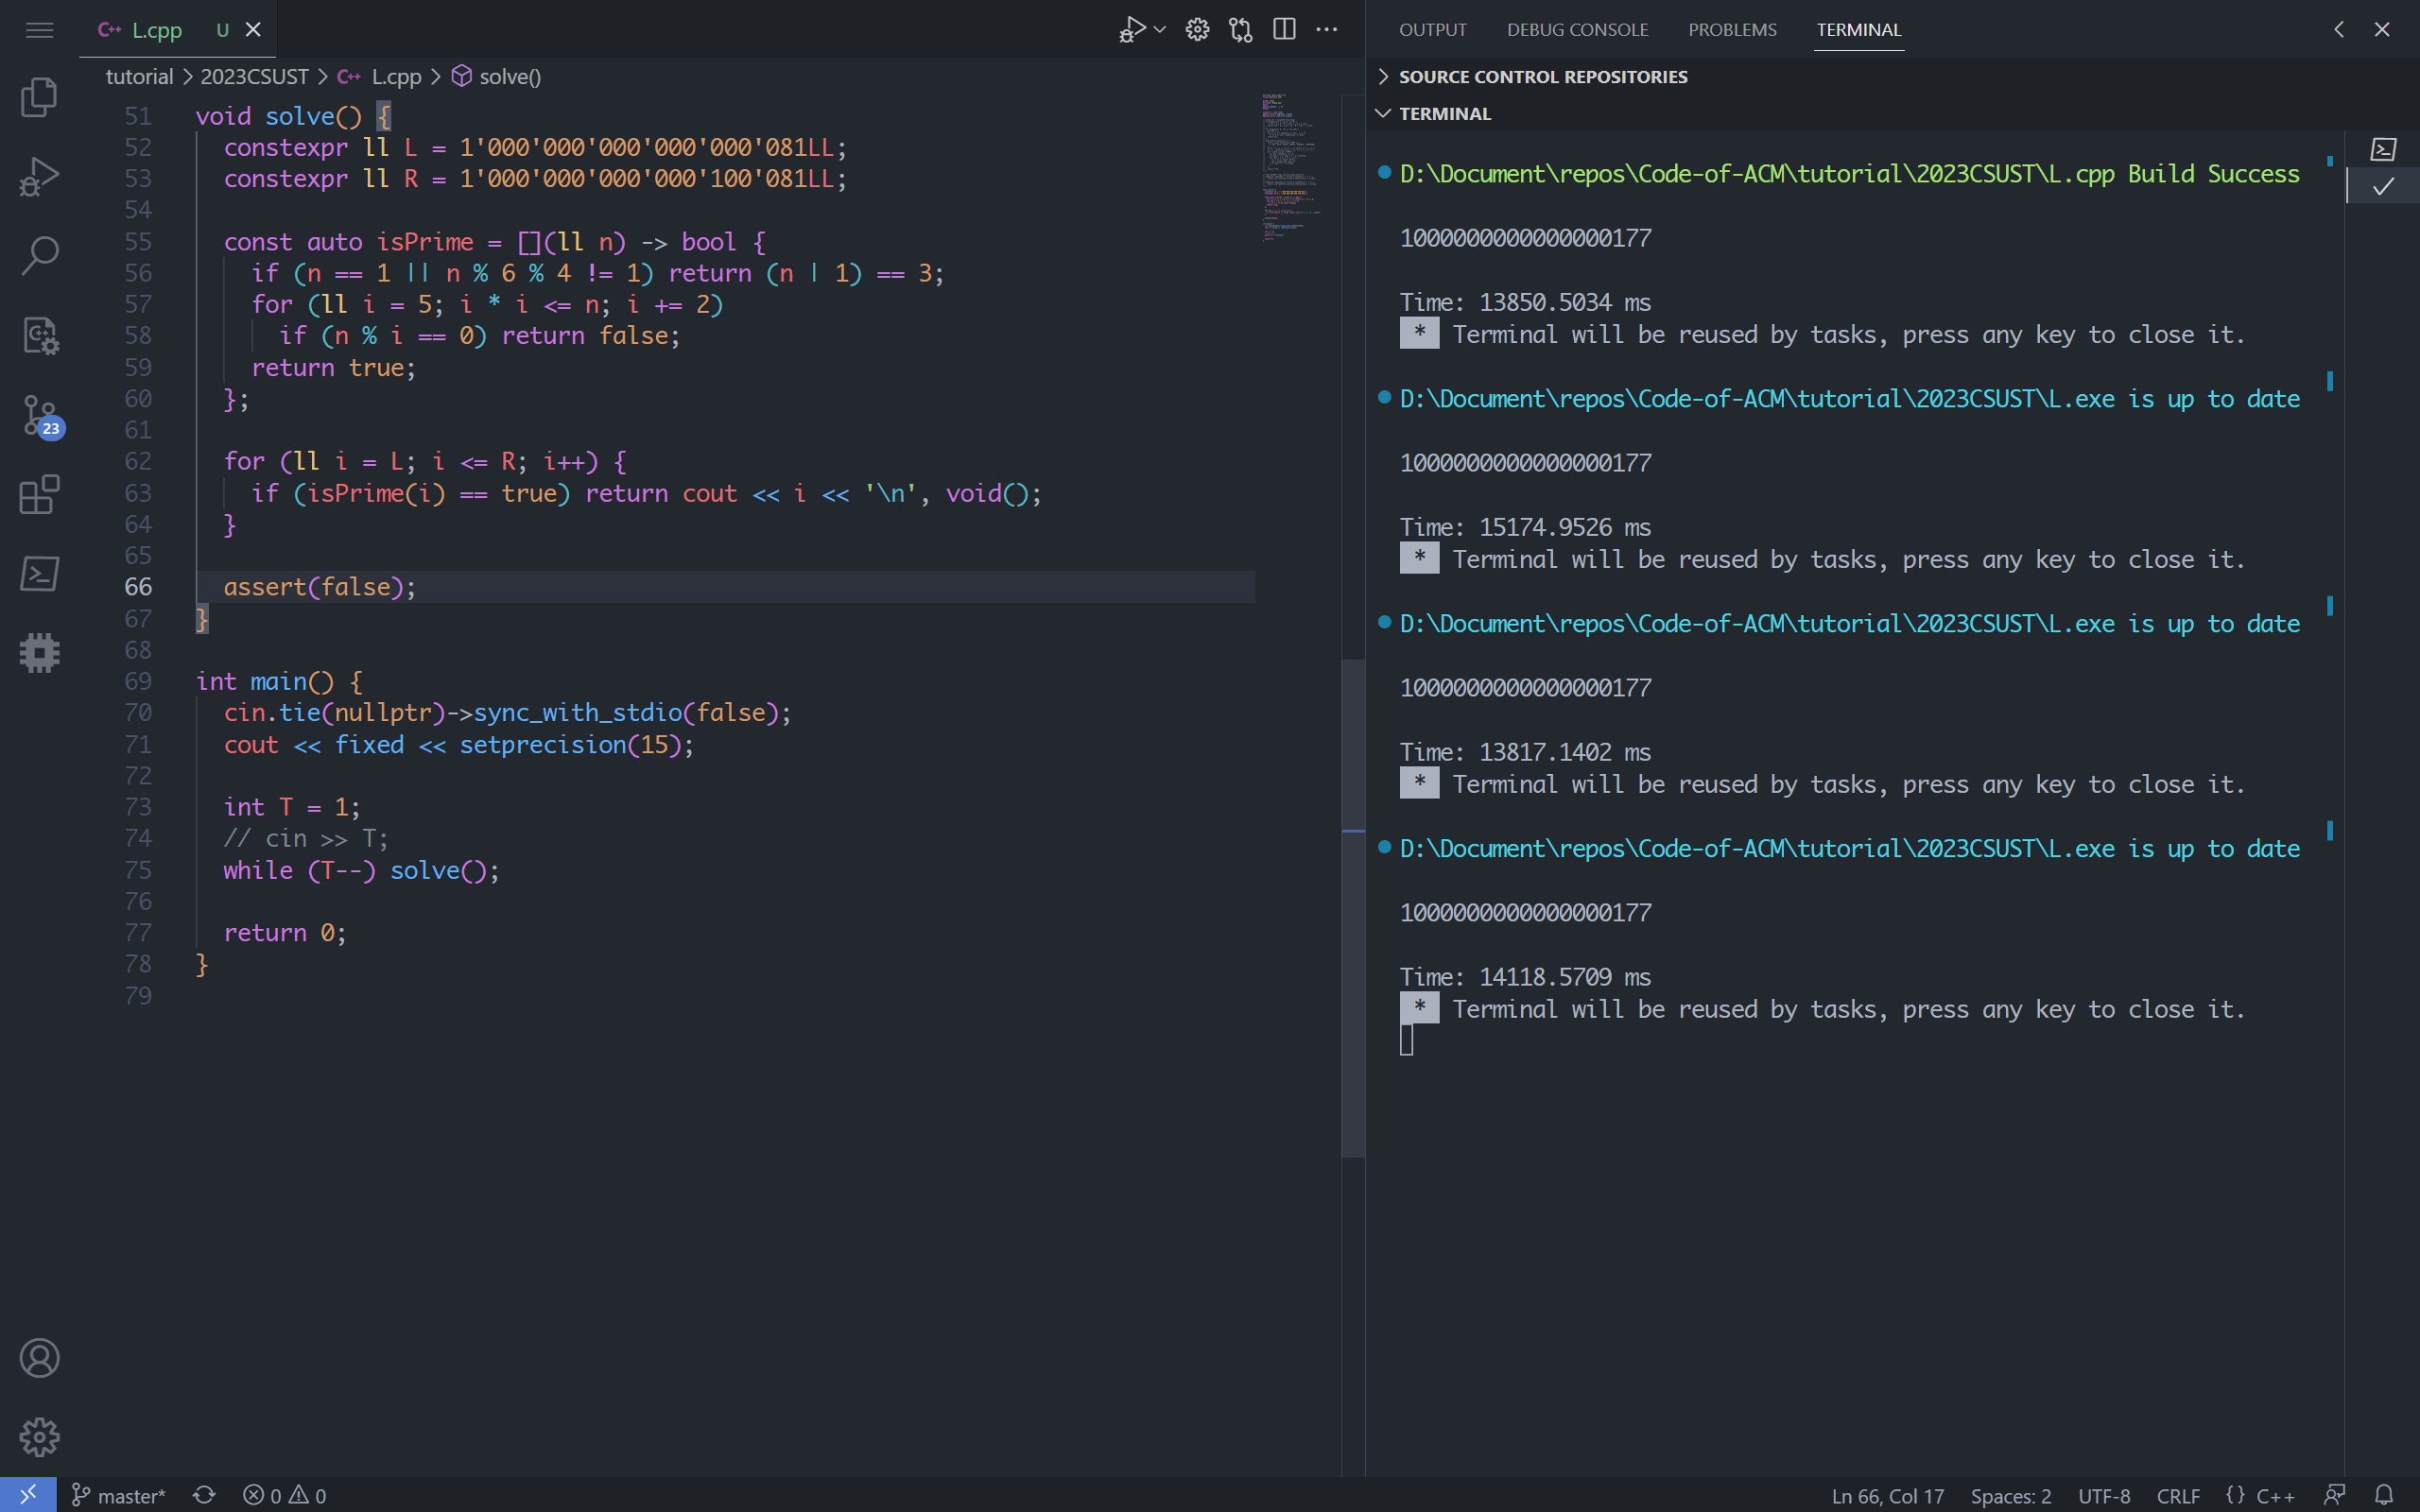
\includegraphics[width=\textwidth]{L.png}
  \caption{试除法$\mathcal{O}(\sqrt{N})$在O2优化的情况下平均用时14s}
  \label{Fig.sqrt}
\end{figure}

\end{document}